
% Template last modified by Jake Hart; please contact course staff if you have any questions regarding using this template

\documentclass[12pt]{article} % You must have the cisXXX .cls file in your project or working directory (i.e. the same directory as this 
\usepackage[legalpaper, portrait, margin=1in]{geometry}
\usepackage[utf8]{inputenc}
%\usepackage{natbib}
\usepackage{graphicx}
\usepackage{cite}
\usepackage{subfigure}
											% Date



\begin{document}

%%%%%%%%%%%%%%%%%%%%%%%%%%%%%%%%%%%%%%%%%%%%%%%%%%%%%%%%%%%%%%%%%%%%%%%%%%%%%%%%%%%%%%%%%

\begin{titlepage}
	\centering
    \vspace{3cm}
    
\includegraphics[scale = 1.5]{figures/MOBI_0.jpg}\\[1.0 cm]	% University Logo,
    \vspace{3cm}
    
    \centering\LARGE{VUB MOBILITY, LOGISTICS \& AUTOMOTIVE TECHNOLOGY RESEARCH CENTRE}
    \vspace{3cm}
	
	\rule{\linewidth}{0.2 mm} \\[0.4 cm]
	{ \huge \bfseries Double Pulse Test MATLAB/Simulink Model}\\
	\rule{\linewidth}{0.2 mm} \\[1.5 cm]
	\vspace{3cm}
	\centering\LARGE{HAKAN POLAT}\\
	\vspace{1cm}
	\centering\large{17 July 2021}
	
	
   
    
    
    
	
\end{titlepage}

%%%%%%%%%%%%%%%%%%%%%%%%%%%%%%%%%%%%%%%%%%%%%%%%%%%%%%%%%%%%%%%%%%%%%%%%%%%%%%%%%%%%%%%%%





\section{Introduction}

Double pulse test (DPT) is a standard test to measure the switching characteristics of a power semiconductor. It has a wide range of applications, ranging from measurement of parasitic capacitances to measuring the turn-on and turn-off losses of the device under test (DUT) for various drain-source voltages $V_{ds}$ and drain-source currents $I_{ds}$. According to \cite{Infineon}, double pulse test allows identifying the technical issues at an earlier stage of the project. Testing the semiconductors under worst-case scenarios allows precautions to be taken, which may cause delays in the timeline.\\

\section{Double Pulse Test}

A DPT circuit consists of a loading inductor, a freewheel diode, and the DUT given in Fig. \ref{fig:DPTcircuit}. Often the same semiconductor is used as a freewheeling diode to measure losses on the body diode. 

\begin{figure}[h!]
	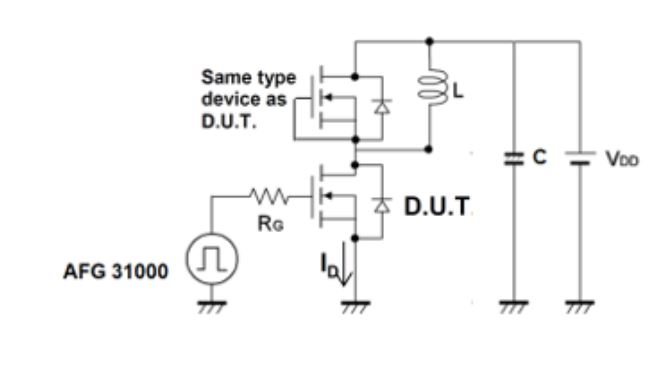
\includegraphics[scale=0.7]{figures/D_P_T.JPG}
	\caption{DPT test circuit.}
	\label{fig:DPTcircuit}
\end{figure}

Therefore, the gate-source voltage ($V_{gs}$) of the high side semiconductor is smaller than the threshold voltage $V_{th}$. To avoid false turn-on during hard switching conditions, a negative voltage is applied for SiC and GaN devices since the parasitic gate-source capacitance ($C_{gs}$) is much smaller than conventional Si devices. The load inductor is first charged to the desired current. Then the DUT is turned off, and the load current flows from the freewheeling body-diode. In order to observe the turn-on characteristics, the DUT is turned on and off once more. By controlling the switching times, the DUT characteristics can be measured in a controlled manner. A typical DUT $I_{ds}$ current is shown in Fig. \ref{fig:DPTtiming} \cite{Infineon}.  Here it is important to list a few features of the load inductor:

\begin{itemize}
    \item The load inductor should not saturate for the currents under testing.
    \item The inductor should be far away from the half-bridge configuration to avoid EMI
    \item The current pulse should be small as possible to avoid heating of the junction, which changes the switching characteristics.
\end{itemize}



\begin{figure}[h!]
	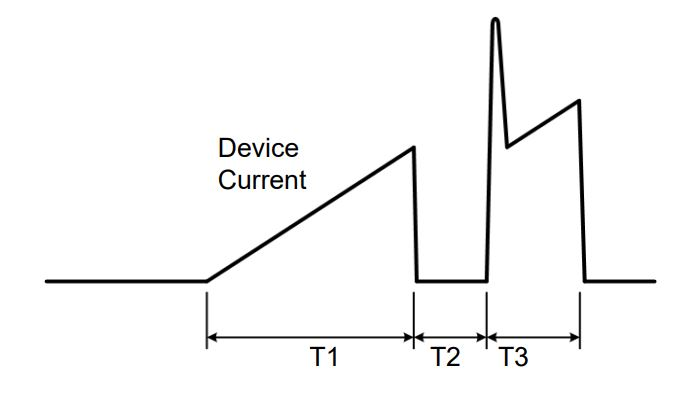
\includegraphics[scale=0.7]{figures/DPT_timing.JPG}
	\caption{DPT DUT $I_{ds}$ representation.}
	\label{fig:DPTtiming}
\end{figure}

\section{Simulink Model}

Prior to real testing, a simulation model is necessary for the initial evaluation of the semiconductor. Therefore, it is essential to model the DPT with DUT in a simulation environment. In this report, a Matlab 2020b/Simulink DPT model is built.\\

The 900~V, 23~A SiC MOSFET with manufacturer part number C3M0120090D is selected as DUT \cite{Cree}. The Simulink model is presented in Fig. \ref{fig:simulinkmodel}. The DC link capacitance is neglected from the model for simplicity. However, during actual experimental testing, the DC-link capacitance should be chosen such that no voltage sags are observed during switching transients. 

\begin{figure}[h!]
	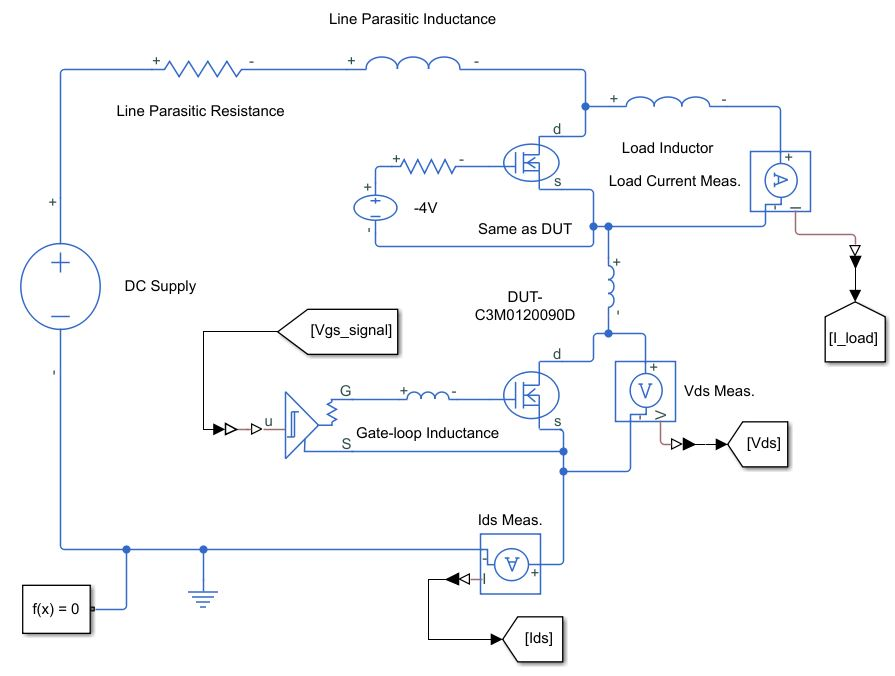
\includegraphics[scale=0.6]{figures/Simulink_circuit.JPG}
	\caption{Simulink DPT model for C3M0120090D SiC MOSFET. }
	\label{fig:simulinkmodel}
\end{figure}

The line parasitic resistance ($R_{par,line}$) and line parasitic inductance ($L_{par,line}$), are parasitic impedances in the AC power loop. Another important parameter is the parasitic inductance between the two semiconductors. This parasitic impedance ($L_{HB}$) is crucial since it directly affects the turn-on and turn-off LC oscillations. For simplicity, it is taken as 1~nH.

\subsection{Gate Driver Parameters}
The gate driver parameters are taken from UCC21530 gate driver, which was given in the reference designs from Texas Instruments \cite{TI}. The gate driver parameters are presented in Table \ref{tab:gatedriverparameters}. The turn on-off voltages are taken from the datasheet presented in \cite{Cree}. The gate loop parasitic inductance is taken as 7~nH, which is an acceptable value in SiC drives. If desired, the parasitic gate loop inductance can be measured using RLC meter with proper PCB measurement probes.

\begin{table}[h]
\centering
\caption{Gate Driver Parameters}
\label{tab:gatedriverparameters}
\begin{tabular}{cc}
\hline \\
Gate Driver model      &   UCC21530-Q1   \\
Turn-on delay time ($t_{on,delay}$)      &   19~ns   \\
Turn-off delay time ($t_{on,delay}$)    &   19~ns    \\
Turn on external gate resistance ($R_on,ext$)    &   5~$\Omega$    \\
Turn-off external gate resistance  ($R_off,ext$)     &   5~$\Omega$   \\
Gate-source turn-on voltage ($V_{gs,on}$) & 15~V\\
Gate-source turn-off voltage ($V_{gs,off}$) & -4~V\\
Gate loop parasitic inductance ($L_{gate}$) & 7~nH\\
\hline
\end{tabular}
\end{table}

\subsection{Semiconductor Model}
The simulink MOSFET model requires the parameters presented in Table \ref{tab:semiconductorparameters}.
\begin{table}[h]
\centering
\caption{C3M0120090D SiC MOSFET Parameters}
\label{tab:semiconductorparameters}
\begin{tabular}{cc}
\hline \\
Semiconductor      &   C3M0120090D SiC MOSFET   \\
Drain-source on state resistance ($R_{ds,on}$)      &   120~$m\Omega$    \\
$I_{ds}$ for $R_{ds,on}$    &   15~A    \\
$V_{ds}$ for $R_{ds,on}$   &   15~V    \\
Gate threshold voltage ($V_{th}$)   &   2.1~V   \\
Input capacitance ($C_{iss}$) & Piecewise linear function wrt. $V_{ds}$\\
Output capacitance ($C_{oss}$) & Piecewise linear function wrt. $V_{ds}$\\
Reverse transfer capacitance ($C_{rss}$) &Piecewise linear function wrt. $V_{ds}$ \\
\hline
\end{tabular}
\end{table}

The parasitic capacitances presented in Table \ref{tab:semiconductorparameters}, are taken as piecewise linear function wrt. the $V_{ds}$. In Fig. \ref{fig:parasiticcapacitance}, the change of the parasitic capacitances is presented. These parameters can also be given as constant. However, the transient response will deviate slightly from realistic results.

\begin{figure}[h!]
\centering	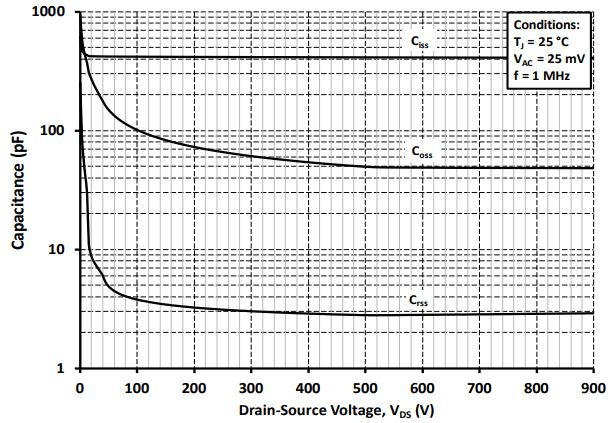
\includegraphics[scale=0.6]{figures/Parasitic_capacitance.JPG}
	\caption{C3M0120090D SiC MOSFET parasitic capacitances with respect to $V_{ds}$.\cite{Cree} }
	\label{fig:parasiticcapacitance}
\end{figure}
\clearpage
\section{Results}
The DPT parameters are listed in Table \ref{tab:DPTpar}. The gate signal ($V_{gate}$), $V_{ds}$, $I_{ds}$ and $I_{load}$ are presented for different parasitic inductances in Fig.~\ref{fig:parasiticswitching}. The turn on and off switchings are presented in Fig.~\ref{fig:parasiticswitching_turnon} and Fig.~\ref{fig:parasiticswitching_turnoff}. The turn on and turn off energies are calculated as 76~$\mu J$, 18~$\mu J$, respectively.

\begin{table}[h]
\centering
\caption{DPT Parameters}
\label{tab:DPTpar}
\begin{tabular}{cc}
\hline \\
Semiconductor      &   C3M0120090D SiC MOSFET   \\
$V_{dc,link}$      &   600~V   \\
$I_{load}$      &   15~A   \\
$L_{load}$      &   1~mH   \\
\hline
\end{tabular}
\end{table}

\begin{figure}[h]
     \centering
     \subfigure[]{
         \centering
        	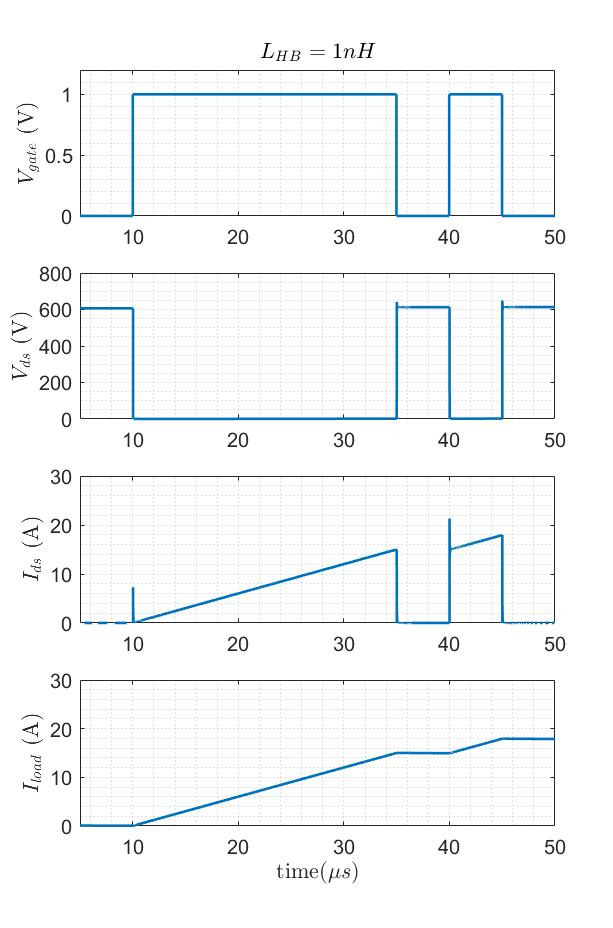
\includegraphics[width=0.45\linewidth]{figures/onenH.jpg}
     }
     \subfigure[]{
         \centering
         	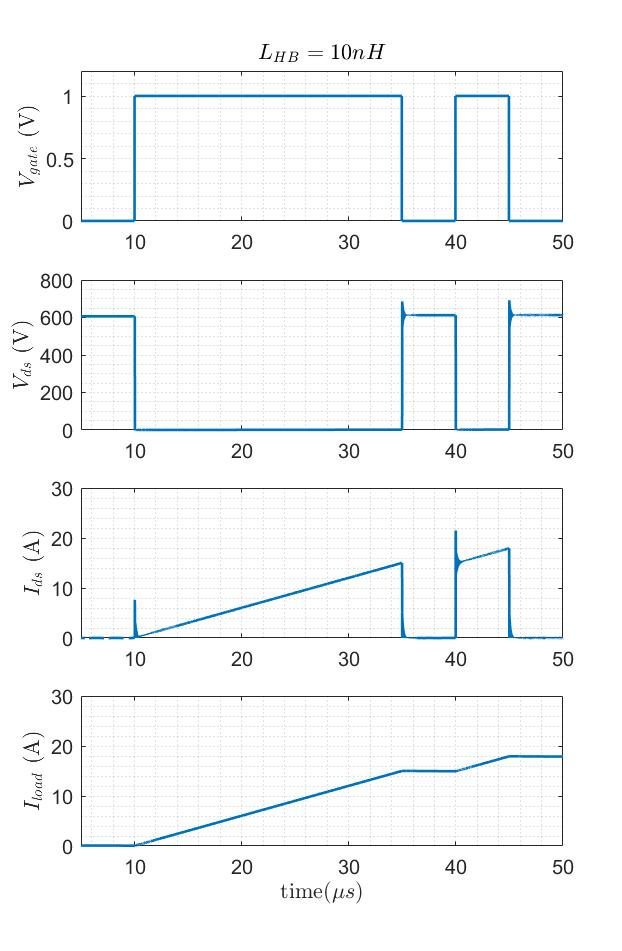
\includegraphics[width=0.45\linewidth]{figures/tenH.jpg}
     }
        \caption{Effect of parasitic inductance on the switching overshoots. Notice the increased oscillation and voltage peak on $V_{ds}$ and $I_{ds}$ during turn on and off.($V_{dc,link}=600V$, $I_{load}=15A$)}
	\label{fig:parasiticswitching}
\end{figure}

\begin{figure}[h]
     \centering
     \subfigure[]{
         \centering
        	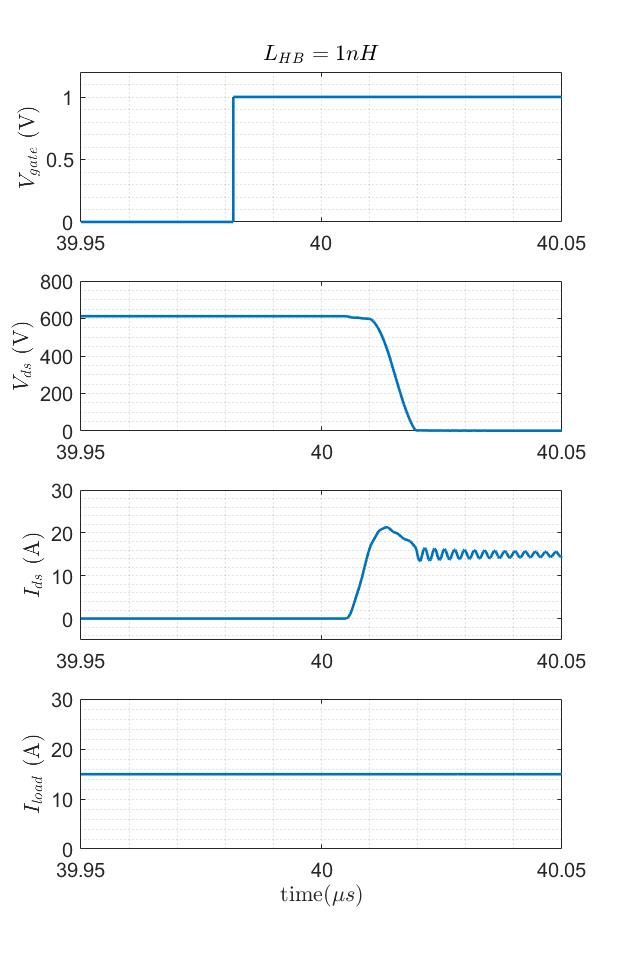
\includegraphics[width=0.45\linewidth]{figures/1nH_turnon.jpg}
     }
     \subfigure[]{
         \centering
         	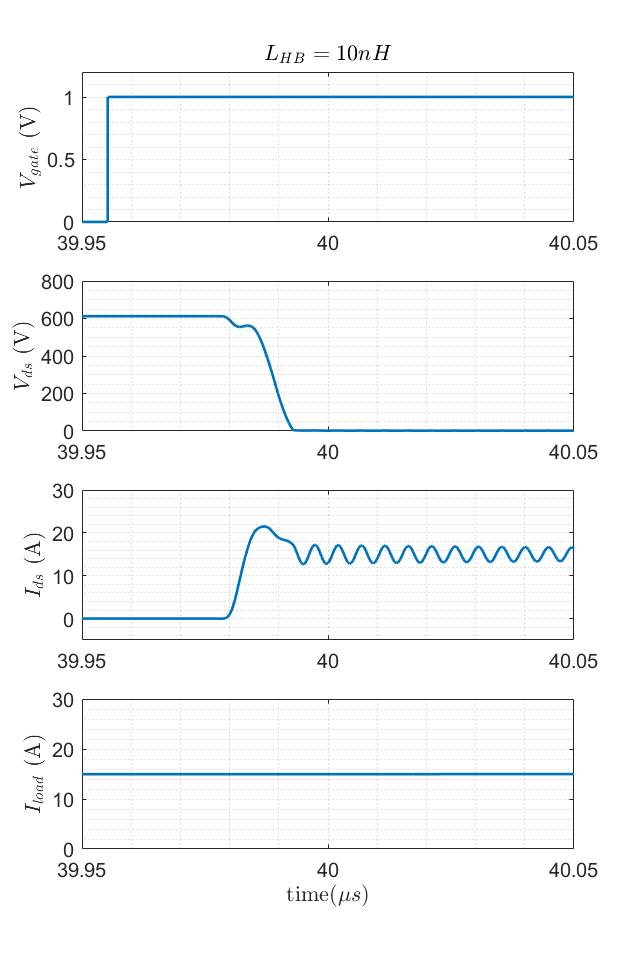
\includegraphics[width=0.45\linewidth]{figures/10nHturnon.jpg}
     }
        \caption{Effect of parasitic inductance on the switching overshoots during turn on. ($V_{dc,link}=600V$, $I_{load}=15A$)}
	\label{fig:parasiticswitching_turnon}
\end{figure}

\begin{figure}[h]
     \centering
     \subfigure[]{
         \centering
        	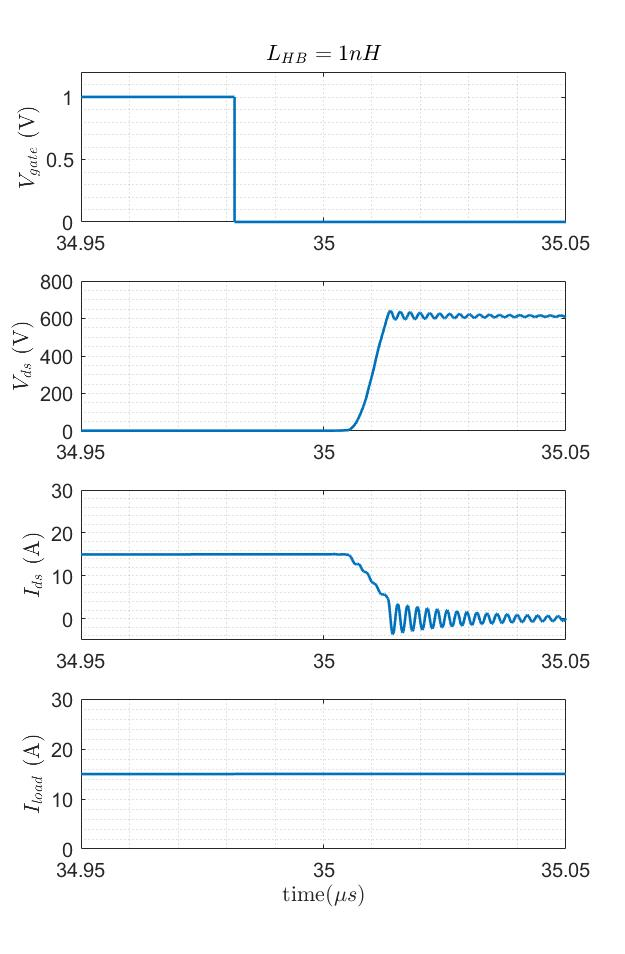
\includegraphics[width=0.45\linewidth]{figures/1nH_turnoff.jpg}
     }
     \subfigure[]{
         \centering
         	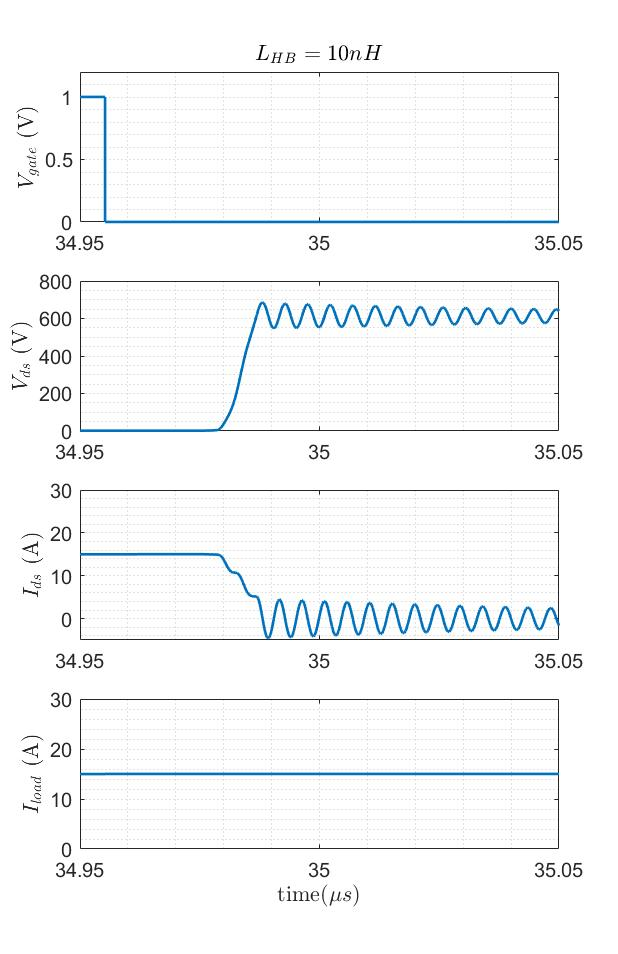
\includegraphics[width=0.45\linewidth]{figures/10nHturnoff.jpg}
     }
        \caption{Effect of parasitic inductance on the switching overshoots during turn off. ($V_{dc,link}=600V$, $I_{load}=15A$)}
	\label{fig:parasiticswitching_turnoff}
\end{figure}
\clearpage

\section{Possible Improvements}

\subsection{GaN Modeling}
Modeling GaN transistors are a bit problematic. While the forward conduction characteristics are like regular MOSFET's the reverse conduction characteristics depend on the applied $V_{gs}$ voltage, and since there is no body diode in a GaNFet \cite{7309716}. Therefore, it is not possible to perfectly model GaNFet using Simulink built-in MOSFET. 

\subsection{SiC Modeling}

The SiC Simulink model can further be improved to improve the transient simulation and experimental agreement. The required parameters can be extracted from manufacturer datasheets using curve fitting functions as in \cite{6941012} and each internal parasitic element can be modeled analytically. 



\section{Short Summary}

In this report, a MATLAB Simulink model is built to simulate a double pulse test for a specific device. While C3M0120090D-Silicon Carbide Power MOSFET is selected as the device under test, by changing the parameters, it is possible to simulate various semiconductors. The found switching losses are lower than the ones presented in the manufacturer's datasheet. This is because of not being able to perfectly model the turn on and off delay times, source/sink currents of the gate driver circuit, or the line parasitic inductance values.

\bibliographystyle{IEEEtran}
\bibliography{ref.bib}
\vfill
\end{document}